%%%%%%%%%%%%%%%%%%%%%%%%%%%%%%%%%%%%%%%%%
% Beamer Presentation
% Ricks Template
%
%
%%%%%%%%%%%%%%%%%%%%%%%%%%%%%%%%%%%%%%%%%

%----------------------------------------------------------------------------------------
%	PACKAGES AND THEMES
%----------------------------------------------------------------------------------------
\documentclass[t,aspectratio=169,11pt,presentation]{beamer}
%\documentclass[t,aspectratio=169,11pt,presentation]{beamer}
%\documentclass[t,aspectratio=169,11pt,draft]{beamer}


% Define colors
\definecolor{ptb5}{RGB}{54,75,154}	 % NT                   
\definecolor{ptb4}{RGB}{74,123,183} % RC + NT	                    
\definecolor{ptb3}{RGB}{110,166,205}                     
\definecolor{ptb2}{RGB}{152,202,225}% EC + RC + NT                  
\definecolor{ptb1}{RGB}{194,228,239}
\definecolor{ptg0}{RGB}{234,236,204}
\definecolor{ptr1}{RGB}{254,218,139} %EC only
\definecolor{ptr2}{RGB}{253,179,102}	                    
\definecolor{ptr3}{RGB}{246,126,75} % AT +	EC + RC                    
\definecolor{ptr4}{RGB}{221,61,45}	 % AT + EC                   
\definecolor{ptr5}{RGB}{165,0,38}	 % AT	   

\usetheme{Boadilla}




% Footer and page numbers

% First remove the navigation symbols from the bottom of all slides 
\setbeamertemplate{navigation symbols}{} 

% Remove the colored line at the bottom
\setbeamertemplate{footline}{}


% Customize items
\setbeamertemplate{itemize items}{\color{ptb2}{\rule[0.05em]{0.6em}{0.6em}}}
\setbeamertemplate{itemize subitem}{\color{ptb2}{\raisebox{0.12em}{$\blacktriangleright$}}}
\setbeamercolor{enumerate item}{fg=black}
\setbeamertemplate{enumerate item}[default]
\setbeamercolor{enumerate subitem}{fg=black}
\setbeamertemplate{enumerate subitem}[default]


\setbeamercolor{subsection in toc}{bg=white,fg=black}




% Table of Contents (if we have one)
\setbeamertemplate{section in toc}{\inserttocsectionnumber.~\inserttocsection}
\setbeamercolor{section in toc}{bg=white,fg=black}
\setbeamertemplate{subsection in toc}{%
  \hspace{1.2em}{{\color{ptb5}{\rule[0.05em]{0.6em}{0.6em}}}~\inserttocsubsection\par}
}
\setbeamercolor{subsection in toc}{bg=white,fg=black}


% Customize beamer colors

\setbeamercolor{titlelike}{fg=white,bg=ptb5}
\setbeamercolor{button}{bg=ptb4,fg=white}
%}

% Nicer looking Itemize and enumerate environments
\newenvironment{wideitemize}{\itemize\addtolength{\itemsep}{14pt}}{\enditemize}
\newenvironment{wideenumerate}{\enumerate\addtolength{\itemsep}{14pt}}{\endenumerate}

% Import packages
\usepackage[default]{lato} % More modern looking font than Helvetica
\usepackage{geometry,caption,color,setspace,dsfont,commath,amsmath,amssymb,bm,mathrsfs}
\usepackage[normalem]{ulem}
\usepackage[comma]{natbib}
\usepackage[short]{optidef}
\usepackage{hhline}
\usepackage{array}
\usepackage{booktabs} % Allows the use of \toprule, \midrule and \bottomrule in tables
\usepackage{adjustbox}
\usepackage{graphicx,xcolor,bbm,xcomment}
\usepackage{appendixnumberbeamer}
\usepackage{textcomp}
\usepackage{colortbl}
\usepackage{subcaption} 
\usepackage{tikz}
\usetikzlibrary{calc,patterns,positioning}
\usepackage{pdflscape}
\usepackage{environ}
\usepackage{array}
\usepackage{accents}
\usepackage{etoolbox}
\usepackage[normalem]{ulem}
\BeforeBeginEnvironment{itemize}{\par}
\BeforeBeginEnvironment{enumerate}{\par}

\bibliographystyle{ecta}

\newcommand*\diff{\mathop{}\!\mathrm{d}}


% Make Section Header Frames
\AtBeginSection[]{

  \setbeamercolor{titlelike}{bg=ptb5,fg=white}
  \setbeamertemplate{navigation symbols}{} 
  \begin{frame}[noframenumbering]
  \vfill
  \centering
  \begin{beamercolorbox}[sep=8pt,center,shadow=true,rounded=true]{title}
    \usebeamerfont{title}\insertsectionhead\par%
  \end{beamercolorbox}
  \vfill
  \end{frame}
  % Make a new prettier page number
\addtobeamertemplate{navigation symbols}{}{%
    \usebeamerfont{footline}%
    \hspace{5em}%
    {\color{black!50}{\small\insertframenumber/\inserttotalframenumber}}%
}
\setbeamercolor{titlelike}{fg=ptb5,bg=white}
}

\AtBeginSubsection[]{
  \setbeamertemplate{navigation symbols}{} 
  \begin{frame}[noframenumbering]
  \vfill
  \centering
  \begin{beamercolorbox}[sep=8pt,center,shadow=false,rounded=true]{title}
    \usebeamerfont{title} \insertsubsectionhead\par%
  \end{beamercolorbox}
  \vfill
  \end{frame}
  % Make a new prettier page number
\addtobeamertemplate{navigation symbols}{}{%
    \usebeamerfont{footline}%
    \hspace{5em}%
    {\color{black!50}{\small\insertframenumber/\inserttotalframenumber}}%
}
}



\tikzset{
    invisible/.style={opacity=0},
    visible on/.style={alt={#1{}{invisible}}},
    alt/.code args={<#1>#2#3}{%
      \alt<#1>{\pgfkeysalso{#2}}{\pgfkeysalso{#3}} % \pgfkeysalso doesn't change the path
    },
  }
  
  
\makeatletter
\newsavebox{\measure@tikzpicture}
\NewEnviron{scaletikzpicturetowidth}[1]{%
  \def\tikz@width{#1}%
  \def\tikzscale{1}\begin{lrbox}{\measure@tikzpicture}%
  \BODY
  \end{lrbox}%
  \pgfmathparse{#1/\wd\measure@tikzpicture}%
  \edef\tikzscale{\pgfmathresult}%
  \BODY
}
\makeatother

\tikzset{
  pics/student/.style args={#1,#2}{
     code={
       \filldraw [fill=#1,draw=black,visible on=#2,line width=1pt] (.1,.3) .. controls (.1,1.4) and (1.4,1.6) .. (1.5,.4) .. controls (1.1,.1) and (.1,0) .. (.1,.3) ;
       \filldraw [fill=#1,draw=black,visible on=#2,line width=1pt] (.7,1.5) circle [radius=.44];
     }
  }
}

%----------------------------------------------------------------------------------------
%	TITLE PAGE
%----------------------------------------------------------------------------------------
 

\title{From Value Added to Welfare Added: \\ A Social Planner Approach to Education Policy and Statistics\vskip.3cm}

\author{Tanner S Eastmond$^1$ \vskip.2cm Nathan Mather$^2$ \vskip.2cm Michael Ricks$^3$ \vskip.2cm Julian Betts$^{1,3}$ }

\begin{document}

\begin{frame}[noframenumbering]
\maketitle
\end{frame}


\setbeamercolor{titlelike}{fg=ptb5,bg=white}
% Make a new prettier page number
\addtobeamertemplate{navigation symbols}{}{%
    \usebeamerfont{footline}%
    \hspace{5em}%
    {\color{black!50}{\small\insertframenumber/\inserttotalframenumber}}%
}



%------------------------------------------------
% Why do we care 
%------------------------------------------------
\begin{frame}[c]{\textbf{What is the effect of a teacher, school, hospital, or policy?} }

\centering
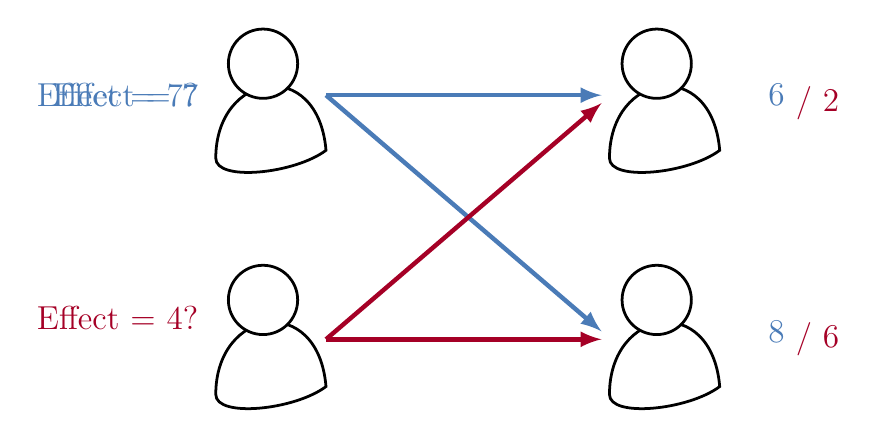
\begin{tikzpicture}[scale=1]
  \draw (-2.5,1.5) pic{student={white,<2->}};
  \node[anchor= east,visible on=<7-10>,font=\large,ptb4] at (-2.5,2.6){Effect = 7 };
  \node[anchor= east,visible on=<12->,font=\large,ptb4] at (-2.5,2.6){Effect = 7?};
  \draw (-2.5,-1.5) pic{student={white,<8->}};
  \node[anchor= south east,visible on=<11->,font=\large,ptr5] at (-2.5,-.5){Effect = 4?};
  \draw (2.5,-1.5) pic{student={white,<2->}};
  \draw (2.5,1.5) pic{student={white,<2->}};
  \draw[-latex,ptb4,ultra thick,visible on=<3->] (-1,2.6) -- (2.5,2.6) node[font=\large,anchor=west,outer sep=2 cm,visible on=<3->]{6}; 
  \draw[-latex,ptb4,ultra thick,visible on=<4->] (-1,2.6) -- (2.5,-.4) node[font=\large,anchor=west,outer sep=2 cm]{8};
  \draw[-latex,ptr5,ultra thick,visible on=<9->] (-1,-.5) -- (2.5,-.5) node[font=\large,anchor=west,outer sep=2.35 cm]{/ 6} ;
  \draw[-latex,ptr5,ultra thick,visible on=<10->] (-1,-.5) -- (2.5,2.5) node[font=\large,anchor=west,outer sep=2.35 cm]{/ 2};
\end{tikzpicture}


\end{frame}

%------------------------------------------------
\begin{frame}{\textbf{Averages ``mean'' well, but don't capture everything} }

\begin{wideitemize}
    \item Whether in teacher value added, school and hospital report cards, or policy evaluations researchers use mean-oriented statistics


    
    \item <2-> But mean masks important heterogeneity of multiple types
    \begin{itemize}
        \item<3->\textbf{Impacts}: If policies have \textbf{\color<3>{ptr3}heterogeneous effects} on different groups 
        % Edu example
        \item<4->\textbf{Outcomes}: If policies affect \textbf{\color<4>{ptr1}multiple outcomes} in different ways
        % Health
        \item<5->\textbf{Preferences}: If policymakers have \textbf{\color<5>{ptr5}heterogeneous value} over groups (e.g., levels and gaps)
        % Public program 
    \end{itemize}

    % The mean statistics do not capture any of these dimensions of heterogeneity
    
    \item<6-> \textbf{\color{ptr5}Theoretically, when does heterogeneity matter for maximizing a social objective?}
  
    \item<7>  \textbf{\color{ptr5}In education policy, how misleading are traditional teacher value added estimates?}
  
\end{wideitemize}

\end{frame}
%------------------------------------------------

%------------------------------------------------
\begin{frame}{\textbf{Emerging evidence suggests heterogeneity matters} }

\begin{wideitemize}
    \item Researchers promote ``value added''-like estimates for policy in many contexts
    %in research and policy with teachers, schools, hospitals, residential care facilities, etc.
        \begin{itemize}
        \item <2-> Heterogeneous and multidimensional value added are the emerging frontier

       {\tiny \color{gray} \citep[]{jackson2018test,pope2017multidimensional,Delgado2020,ahn2021importance,bates2022teacher,Dahlstrand2022defying}}

       \item<3->But both heterogeneity and multidimensionality undermine ranking units and allocations
    
        {\tiny \color{gray} \citep[]{condie2014teacher}}
        \end{itemize}
    
    
    \item<4-> In the real world, numerous policies have distributional objectives 
        \begin{itemize}
        % No Child Left Behind, means-tested public programs, progressive taxation, etc.
        \item<5-> Heterogeneous weights from public finance can extend to cost-benefit analysis
        
        {\tiny \color{gray} \citep[]{adler2016benefit,fleurbaey2016use}}
        \item<6-> Can welfare theory also make value added useful despite heterogeneity?
    \end{itemize}

    
   
\end{wideitemize}

\end{frame}
%------------------------------------------------
%------------------------------------------------
\begin{frame}{\textbf{The key is moving from value added to ``welfare-added''} }

\begin{wideitemize}
    \item We use a welfare-theoretic framework to approach a policymaker's objective
    %in research and policy with teachers, schools, hospitals, residential care facilities, etc.
        \begin{itemize}
            \item<2-> Framework fully ranks allocations, given weights on outcomes and groups 
            \item<3-> We characterize three gains from including heterogeneity in estimation
    \end{itemize}
    \vspace{12pt}
\end{wideitemize} 
    
    \begin{wideenumerate}
    \item<4-> Using \textbf{\color<4-5>{ptr3}comparative advantage} makes better allocations than only absolute
    \begin{itemize}
        \item<5-> Related to literatures on targeting for health and public programs
    \end{itemize}
    \item<6-> Directly addressing distributional or \textbf{\color<6-7>{ptr5}equity concerns} controls relevant gaps
    \begin{itemize}
        \item<7-> As in research in optimal tax, discrimination, and environmental justice 
    \end{itemize}
    \item<8-> Heterogeneous estimators may be more \textbf{\color<8-9>{ptb3}externally valid}
    \begin{itemize}
        \item<9-> Like papers on drug trials and selection on unobservables
    \end{itemize}
    \end{wideenumerate}

\end{frame}


%------------------------------------------------
%------------------------------------------------
\begin{frame}{\textbf{We apply this theory of heterogeneity to teacher value added} }

\begin{wideitemize}
    \item We estimate \textbf{\color<2-3>{ptr3}heterogeneous}, \textbf{\color<4-5>{ptr1}multidimensional} value added in San Diego Unified
    \begin{itemize}
        \item Over 1,700 teachers in 3-5th grade classrooms between 2002-2013
    \end{itemize}
    \item<7-> We focus on \textbf{\color<7-11>{ptr3}achievement} impacts on \textbf{\color<7-11>{ptr1}multiple subjects}

    \item<12-> We find substantial, persistent heterogeneity (with some correlation within teachers)
    %in research and policy with teachers, schools, hospitals, residential care facilities, etc.
\end{wideitemize} 

\centering
\vspace{12pt}
\begin{tikzpicture}
   
\tikzstyle{box}=[rectangle,thick,draw=black,outer sep=0pt,minimum width=3.7cm,minimum height=1.cm,align=center,font=\fontsize{10pt}{10pt}\selectfont]

\node (B1) at (0,0) [box,label={[align=center,anchor=south,visible on=<5>,ptr1]\textbf{Outcome 1}},label={[align=center,anchor=south,visible on=<6->,]\textbf{Outcome 1}},anchor=south east,visible on=<3->] {};
\node (B2) at (B1.east) [box,label={[align=center,anchor=south,visible on=<5>,ptr1]\textbf{Outcome 2}},label={[align=center,anchor=south,visible on=<6->]\textbf{Outcome 2}},anchor=west,visible on=<3->] {};
\node (B3) at (B1.south)  [box,anchor=north,visible on=<3->] {};
\node (B4) at (B1.south east) [box,anchor=north west,visible on=<3->] {};
\node (O1) at (B4.east) [box,draw=none,anchor= west,minimum width=2.5cm] {};


\node (C1) at (0,0) [box,anchor=south east,visible on=<8->] {\textbf<8>{High Achieving Math}} ;
\node (C2) at (C1.east) [box,anchor= west,visible on=<9->] {\textbf<9>{High Achieving ELA}} ;
\node (C3) at (C1.south)  [box,anchor=north,visible on=<10->] {\textbf<10>{Low Achieving Math}};
\node (C4) at (C1.south east) [box,anchor=north west,visible on=<11->] {\textbf<11>{Low Achieving ELA}};


\node (T1) at (B1.west) [rectangle,draw=none,visible on=<3->,outer sep=1pt,align=right,anchor=east,minimum width=2.3cm] {\color<3>{ptr3}\textbf{Group A}};
\node (T2) at (B3.west) [rectangle,draw=none,visible on=<3->,outer sep=1pt,align=right,anchor=east,minimum width=2.3cm] {\color<3>{ptr3}\textbf{Group B}};
\end{tikzpicture}


\end{frame}



%------------------------------------------------
%------------------------------------------------
\begin{frame}{\textbf{Heterogeneity is key for using teachers' skills effectively}}

    \begin{wideitemize}
    \item We reallocate teachers within (across) schools based on our estimates of value added
    \begin{itemize}
        \item<2-> How do allocations compare to the results to using traditional estimates 
    \end{itemize}
    \end{wideitemize}
    \vspace{12pt}
    \begin{wideenumerate}
    \item<3-> Heterogeneous VA raises average scores 34-50\% (66-97\%) more than traditional VA
    \begin{itemize}
        \item<4-> The across-school gains are 0.04$\sigma$ in ELA and 0.06$\sigma$ in Math

         {\tiny \color{gray} \citep[]{bates2022teacher}}
    \end{itemize}
    \item<5-> With distributional concerns, heterogeneous VA boosts average scores by 16-50\% 
    %(similar welfare)
    \begin{itemize}
        \item<6-> Reallocations close gaps, but only moving teachers across discticts shrink racial gaps
    \end{itemize}    
    \item<7-> Combined optimization could increase present valued earnings by \$8.6 M (\$32.5 M) 
    \begin{itemize}
        \item<9-> Only enormous costs to teachers/parents/admins/union rationalize status quo
    \end{itemize}
    \end{wideenumerate}

\end{frame}

\setbeamertemplate{navigation symbols}{} 
  
%-----------------------------------------------
\begin{frame}[c,noframenumbering]{Today's Talk}

\begin{columns}
\begin{column}{0.575\textwidth}
\vspace{-1.5em}
\begin{wideenumerate}
    \item When Will Heterogeneity Matter for Welfare?
    \begin{itemize}
        \item Absolute and Comparative Advantage
        \item Distributional Concerns
        \item A Note on Estimation
    \end{itemize}
    \item What Are the Implications for Value Added?
    \begin{itemize}
        \item Heterogeneous Impacts
        \item Reallocations and Decompositions
    \end{itemize}
    \item What About Welfare and Policy?
\end{wideenumerate}
\end{column}
\begin{column}{0.40\textwidth}
\vspace{-1.5em}

\begin{tikzpicture}
%\draw[line width=.5cm] (0,0)  -- (3.2,1.8) -- (0,3.5) -- (3,4.2);
\usetikzlibrary{arrows}
\usetikzlibrary{shapes}
\tikzstyle{every node}=[draw=black,fill=black, ellipse]
\node[minimum width=2.6cm, minimum height = 1cm] (a) at (0,0) {};
\node[minimum width=2cm, minimum height = .8cm] (b) at (4,1.6) {};
\node[minimum width=1.6cm, minimum height = .6cm] (c) at (0,3.2) {};
\node[minimum width=1.2cm, minimum height = .4cm] (d) at (3.2,3.9) {};
\draw[fill = black] (a.75) -- (b.188) -- (b.235) -- (a.06);
\draw[fill = black] (b.170) -- (c.318) -- (c.348) -- (b.140);
\draw[fill = black] (c.5) -- (d.205) -- (d.182) -- (c.28);
\draw[fill = black]  (2.8,5.5) to  [bend right=14] (3.2,4.6) to [bend right =14] (3.6,5.5) -- cycle;
\draw[fill = black] (3.6,5.5) arc (0:180:.4cm);
\draw[fill = white] (3.2,5.5) circle (.22cm);

\end{tikzpicture}



\end{column}
\end{columns}
\end{frame}


\addtobeamertemplate{navigation symbols}{}{%
    \usebeamerfont{footline}%
    \hspace{5em}%
    {\color{black!50}{\small\insertframenumber/\inserttotalframenumber}}%
}

%------------------------------------------------
\section{When Will Heterogeneity Matter for Welfare?}

\begin{frame}{\textbf{A welfare framework for using value added}}
\begin{wideitemize}
    \item Assume a social planner has some objective $\mathcal{W}^j$ that depends on policy $j$
\end{wideitemize}\vspace{-6pt}
\begin{align*}  
      \only<1-2>{\mathcal{W}^j &=  \int_0^1 \psi^j_i U^j_i \text{d}i \\}%
      \only<3-6>{\accentset{\sim}{\mathcal{W}}^j &=  \int_0^1 \psi^j_i S(Y^j_i,X^j_i) \text{d}i \\}%
      \only<7->{\Delta \accentset{\sim}{\mathcal{W}}^j  &=  \int_0^1 \omega_i(S^j_i,S^0_i) \Delta S^j_i \text{d}i \\}%
      \color{white} \sum  & \color{white}\sum \sum \sum  \sum \sum \sum \sum 
\end{align*}\vspace{-24pt}
\begin{wideitemize}
    \item<2-> With unobserved utility, policymakers ``score'' allocations based on observed outcomes
    \begin{itemize}
        \item<4-> Using the score will be the key insight for overcoming \textbf{\color<4>{ptr1}multidimensionality}
        \item<5-> We're agnostic about the score, but includes nice options like ``surrogate indices''

    {\tiny \color{gray} \citep[]{finkelstein2019take}}
    \end{itemize}
    
        \item<6-> Without spillovers, the score will explain the welfare effects of any policy
        
    \hyperlink{proof1}{\beamerbutton{Proof}}
        \begin{itemize}
        \item<8-> Welfare weights $\omega_i$ capture the social value of $i$'s score increase 
        \item<9-> Using these weights will be the key insight for overcoming \textbf{\color<9>{ptr3}heterogeneity}
    \end{itemize}
    
\end{wideitemize}
    
\end{frame}


\begin{frame}{\textbf{Value added, welfare, and comparative advantage}}
\begin{wideitemize}
    \item Consider policies that involve assigning different units to different ``treatments'' $d$
 
    \item<2-> Imagine using the population average treatment effect $\tau^d_{ATE}=\mathbb{E}[S^d-S^0]$ to forecast the welfare of a given allocation: $\tilde{\tau}^j \equiv \int_i \sum_d \omega_i  p^j(d,i) \tau^d_{ATE} \text{d}i$
\begin{itemize}
    \item<3-> Under the same assumptions, the projected welfare is biased
    
    \hyperlink{proof2}{\beamerbutton{Proof}}
   
 \end{itemize}   \vspace{-12pt}
    \begin{align*}
     \only<3->{    \text{\textbf{Bias}}^j_1 &= \Delta \accentset{\sim}{\mathcal{W}}^j - \tilde{\tau}^j \\
                        &= \int_i \sum_d \omega_i p^j(d,i) (\Delta S^j_i-\tau^d_{ATE})\text{d}i \color{white} \sum \sum \sum}
    \end{align*}



%\item<3-> Assuming heterogeneity on observables, $\mathcal{X}$, the projected welfare is biased:
% \end{itemize}   
%    \begin{align*}
%         \text{\textbf{Bias}}^j &= \Delta \accentset{\sim}{\mathcal{W}}^j - \tau^j_{ATE} \\
%                        &= \int_\mathcal{X} \sum_d \omega(x) p^j(d,x) (\tau^d_{CATE}(x)-\tau^d_{ATE})\text{d}x
%    \end{align*}
    % Note int_x ( t(x) f(x|d) p^d -t p^d + ... for all d) dx 
  

     \item<5-> \textbf{\color<5>{ptr3}Comparative advantage} means $\tau^d_{ATE}$ is not \textbf{\color<5>{ptb3}externally valid} everywhere
       \begin{itemize}
  \item<6-> Bias is zero only when not assigned by \textbf{\color<6>{ptr3}comparative advantage} on average
  
  \item<7-> \textbf{\color{ptb3}External validity} concerns are exacerbated when you have to estimate $\tau^d$
  
            \hyperlink{proof2}{\beamerbutton{Details}}
       \end{itemize} 

    
        
    
\end{wideitemize}
    
\end{frame}



\begin{frame}{\textbf{Value added, welfare, and distributional concerns}}
\begin{wideitemize}
    \item Complications arise from not knowing $\tau^j_{ATE} = \mathbb[S^j-S^0]$, but what if we did?
     \begin{itemize}
        \item<2-> For example, consider the estimate $\bar{\omega} \tau^j_{ATE}$ from \citet{Keyser_2020}
     \end{itemize}

    \item<3-> Under the same assumptions, the projected welfare is still biased
    
    \hyperlink{proof3}{\beamerbutton{Proof}}
    \vspace{-12pt}
    \begin{align*}
     \only<3->{    \text{\textbf{Bias}}^j_2 &= \Delta \accentset{\sim}{\mathcal{W}}^j - \bar{\omega} \tau^j_{ATE} \color{white} \sum \sum \sum\\
                        &= \text{Cov}(\omega_i,\Delta S^j_i) }
    \end{align*}    
        
    \item<4-> Means aren't enough if \textbf{\color<4>{ptr5}distributional concerns} interact with heterogeneity 
    \begin{itemize}
        \item Some conditions can only guarantee zero bias, e.g., if there is no heterogeneity or if the objective is to raise average scores 
    \end{itemize}
    
\end{wideitemize}
    
\end{frame}



\begin{frame}{\textbf{How close can you get with heterogeneity?}}
\begin{wideitemize}
    \item Knowing the full joint distribution of individual-level effects and weights is unlikely
 \begin{itemize}
     \item In welfare theory and empirical research, the solution is to use characteristics $\mathcal{X}$
 \end{itemize}

\item<2-> Assuming all heterogeneity is on observables, the projected welfare is unbiased:
\begin{itemize}
    \item Where the conditional average effect of $d$ is $\tau^d_{CATE}(x)=\mathbb{E}[S^d-S^0|X]$
\end{itemize}
    \begin{align*}
         \Delta \accentset{\sim}{\mathcal{W}}^j &= \int_\mathcal{X} \sum_d \omega(x) p^j(d,x) \tau^d_{CATE}(x)\text{d}x
    \end{align*}
     \item<3-> Even if missing a relevant $x$, conditioning will shrink the bias under certain conditions
     \begin{itemize}
         \item Similar to intuition for how regression controls affect omitted variable bias
     \end{itemize}
    \begin{align*}
     \text{\textbf{Bias}}^j_1 &= \int_i \omega_i p^j(d,i) (\Delta S^j_i-\tau^d_{CATE}(x_i))\text{d}i  \\
     \text{\textbf{Bias}}^j_2 &= \int_\mathcal{X} \text{Cov}(\omega_i,\Delta S^j_i|x) \text{d}x 
    \end{align*}  

       

\end{wideitemize}
    
\end{frame}




\begin{frame}[c]{\textbf{Each component could matter substantially for welfare}}
\centering
\resizebox{!}{.46\textwidth}{
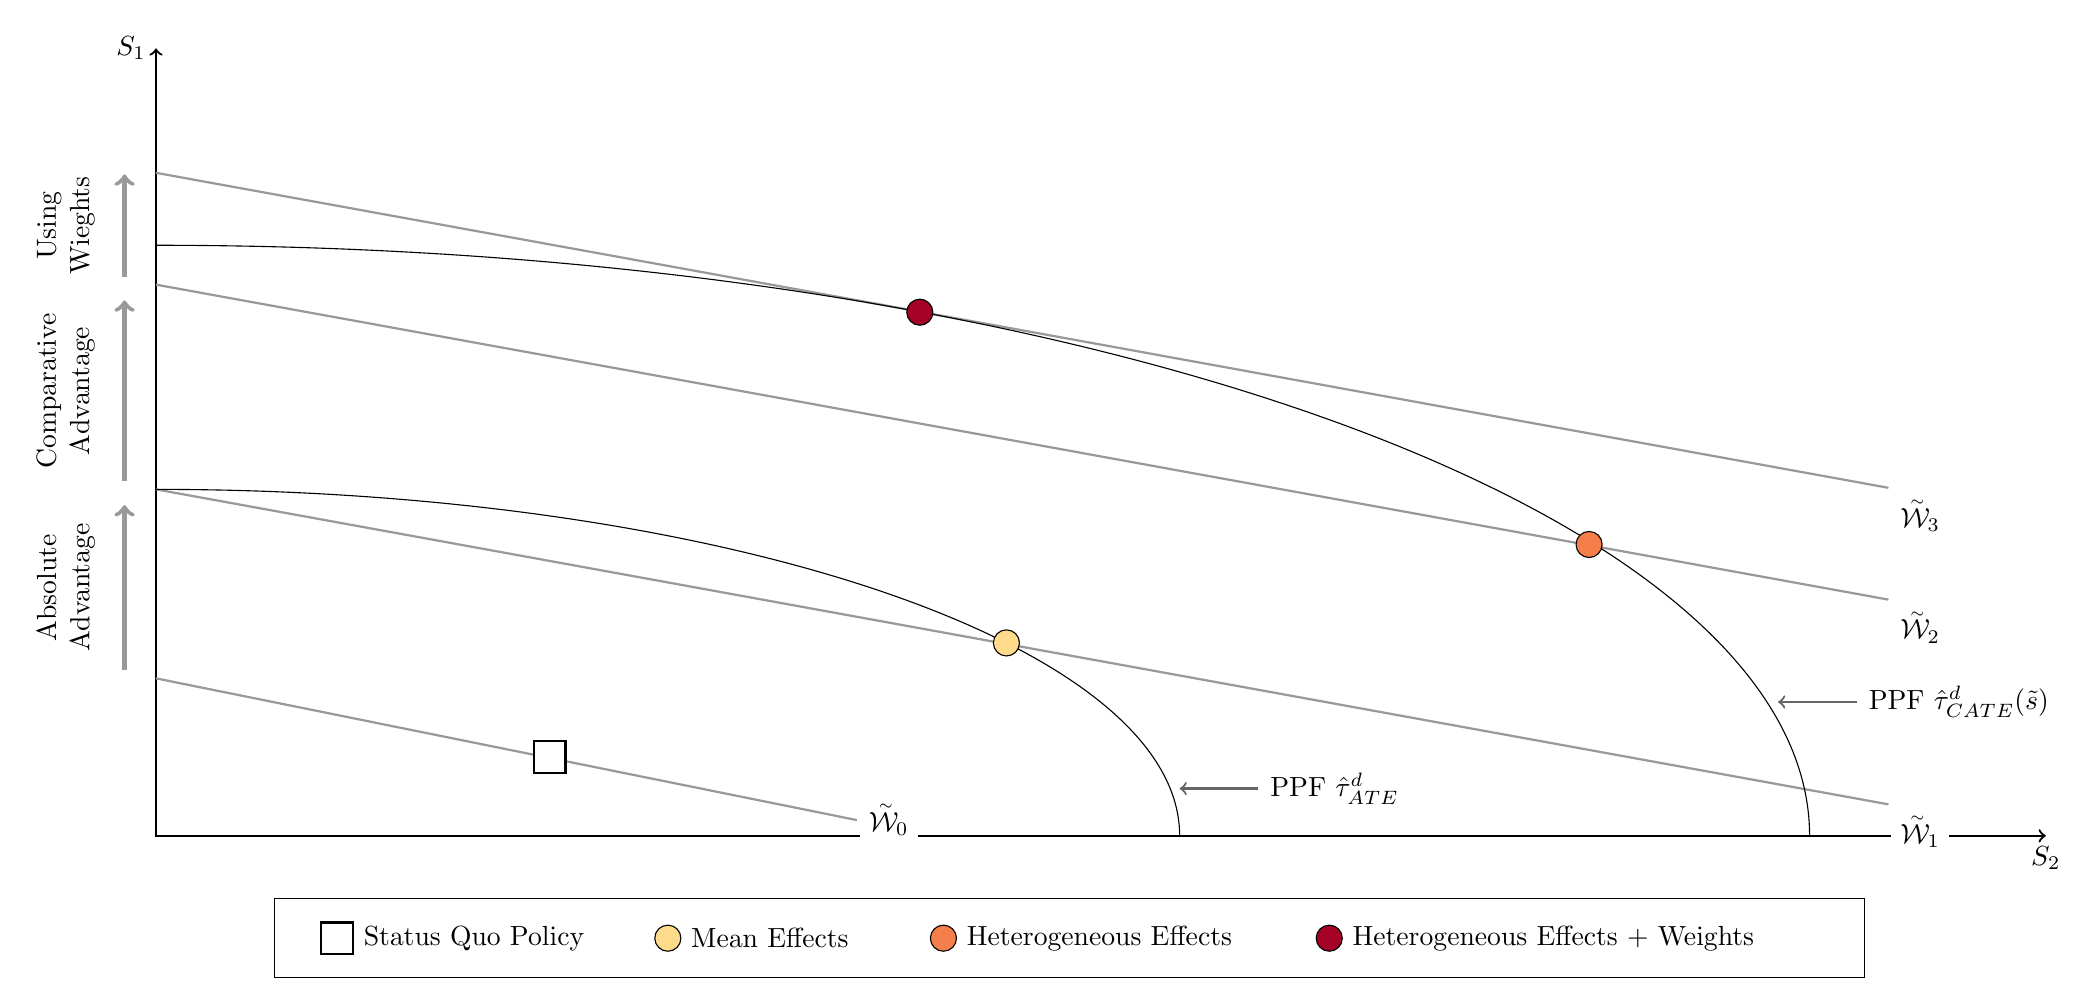
\begin{tikzpicture}[scale=1]
	\draw[thick,<->] (0,10) node[left]{$S_1$} --(0,0)--(24,0) node[below]{$S_2$};
	\draw[dashed,color=black!40,visible on=<13-20>] (0,8.42)--(22,4.42) node[anchor=north west,fill=white,text=black,outer sep=1pt]{$\accentset{\sim}{\mathcal{W}}_3$};
	\draw[dashed,color=black!40,visible on=<11->] (0,7)--(22,3) node[anchor=north west,fill=white,text=black,outer sep=1pt]{$\accentset{\sim}{\mathcal{W}}_2$};
	\draw[dashed,color=black!40,visible on=<10->] (0,4.4)--(22,.4) node[anchor=north west,fill=white,text=black,outer sep=1pt]{$\accentset{\sim}{\mathcal{W}}_1$};
	\draw[dashed,color=black!40,visible on=<9->] (0,2)--(8.9,.2) node[anchor=west,fill=white,text=black,outer sep=1pt]{$\accentset{\sim}{\mathcal{W}}_0$};
	\draw[thick,color=black!40,visible on=<14-15>] (0,2)--(8.9,.2);
    \draw[thick,color=black!40,visible on=<14-17>] (0,4.4)--(22,.4);
    \draw[thick,color=black!40,visible on=<16-19>] (0,7)--(22,3);
    \draw[thick,color=black!40,visible on=<18-19>] (0,8.42)--(22,4.42);
	\draw[visible on=<5->] (21,0) arc(0:90:21cm and 7.5cm);
	\draw[visible on=<3->] (13,0) arc(0:90:13cm and 4.4cm);
	\node[fill=white, draw=black,thick,minimum width=.4cm,minimum height=.4cm,visible on=<2->] at (5.,1) {};
	\node[fill=ptr1, circle, draw=black,visible on=<4->] at (10.8,2.45) {};
	\node[fill=ptr3, circle, draw=black,visible on=<6->] at (18.2,3.7) {};
	\node[fill=ptr5, circle, draw=black,visible on=<13->] at (9.7,6.65) {};
	\draw[thick,<-,color=black!60,visible on=<3->] (13,.6)--(14,.6) node[anchor= west,fill=white,text=black,outer sep=1pt]{PPF $\hat{\tau}^d_{ATE}$};
	\draw[thick,<-,color=black!60,visible on=<5->] (20.6,1.7)--(21.6,1.7) node[anchor= west,fill=white,text=black,outer sep=1pt]{PPF $\hat{\tau}^d_{CATE}(\tilde{s})$};
	\draw[ultra thick, ->,color=black!40,visible on=<15->](-.4,2.1)-- node [midway, left,rotate=90,color=black,anchor=north,outer sep=-35pt,align=center] {Absolute \\ Advantage}(-.4,4.2) ;
	\draw[ultra thick, ->,color=black!40,visible on=<17->](-.4,4.5)-- node [midway, left,rotate=90,color=black,anchor=north,outer sep=-35pt,align=center] {Comparative \\ Advantage}(-.4,6.8) ;
	\draw[ultra thick, ->,color=black!40,visible on=<19->](-.4,7.1)-- node [ left,rotate=90,color=black,anchor=north,outer sep=-35pt,align=center] {Using \\ Wieghts}(-.4,8.4) ;
    \draw[color=black] (1.5,-.8) --(21.7,-.8) --(21.7,-1.8) --(1.5,-1.8) --  (1.5,-.8);
	\node[fill=white, draw=black,thick,label=0:Status Quo Policy,minimum width=.4cm,minimum height=.4cm,visible on=<2->] at (2.3,-1.3) {};
	\node[fill=ptr1, circle, draw=black,label=0:Mean Effects,visible on=<4->] at (6.5,-1.3) {};
	\node[fill=ptr3, circle, draw=black,label=0:Heterogeneous Effects,visible on=<6->] at (10,-1.3){};
	\node[fill=ptr5, circle, draw=black,label=0:Heterogeneous Effects + Weights,visible on=<13->] at (14.9,-1.3)  {};
	%\draw[color=black] (7.5,-.8) --(18,-.8) --(18,-2.6) --(7.5,-2.6) --  (7.5,-.8);
	%\node[fill=white, draw=black,thick,label=0:Status Quo Policy,minimum width=.4cm,minimum height=.4cm,visible on=<2->] at (8.5,-1.3) {};
	%\node[fill=ptr1, circle, draw=black,label=0:Mean Effects,visible on=<4->] at (13.7,-1.3) {};
	%\node[fill=ptr3, circle, draw=black,label=0:Het Effects,visible on=<6->] at (8.5,-2.05){};
	%\node[fill=ptr5, circle, draw=black,label=0:Het + Weights,visible on=<13->] at (13.7,-2.05)  {};
\end{tikzpicture}}
\end{frame}


\section{Application: Welfare and Heterogeneous Value Added}

\subsection{Estimating Heterogeneous Teacher Value Added}



\begin{frame}[label=va]{\textbf{Estimating value added in San Deigo Unified}}
\begin{wideitemize}
    \item Empirical setting is the San Diego Unified School District
    \begin{itemize}
        \item Second largest district in CA, broadly representative of the state
        \item 1,791 teachers in grades 3-5 classrooms from 2002-2013
    \end{itemize}

    \item<2-> We explore \textbf{\color<2>{ptr3}heterogeneity in value added} along the achievement distribution
    \begin{itemize}
        \item<3-> Achievement seems like the most natural dimension of \textbf{\color<3>{ptr3}heterogeneity in teacher effects} (think: teaching differentiation) and \textbf{\color<3>{ptr5}social preferences} (think: policy examples)
        \item<4-> Split estimates by median score in the district separately for \textbf{\color<4>{ptr1}math and ELA}
    \end{itemize}
    

    \item<3-> Very standard VA estimation adapted for heterogeneity following \citet{chetty2014measuring1}, \citet{Delgado2020}, and \citet{bates2022teacher}
    
    \hyperlink{details}{\beamerbutton{VA Estimation Details}}      
 \begin{itemize}
        \item<5-> \textbf{Key Assumption:} classroom-by-achievement-type shocks and idiosyncratic shocks are conditionally independent (with restrictions about stationarity)
    \end{itemize}


\end{wideitemize}
\end{frame}



\begin{frame}[c]{\textbf{Teacher effects are correlated but dispersed}}
\centering
 \includegraphics[width=.95\textwidth]{Working_Slides/WS_Figures/02a_VA.pdf}%
\end{frame}


\begin{frame}[label=effects]{\textbf{Estimation extensions and robustness checks}}
\begin{wideitemize}
    \item Heterogeneous effects leave lots of room for \textbf{\color<1>{ptr3}comparative advantage}
    \begin{itemize}
        \item Cross subject correlations are weaker than within-subject correlations

        \hyperlink{cross}{\beamerbutton{Cross-Subject Scatter}}
        \item Similar to cross-race correlation and less correlated than cross-SES
        
         {\tiny \color{gray} \citep[]{Delgado2020,bates2022teacher}}
    \end{itemize}

    \item<2->\textbf{\color<2>{ptr5}Key Concern}: Are the differences noise or actual comparative advantage?

    \item<3-> Heterogeneity seems to reliably estimate economically meaningful differences
    
        \hyperlink{persistence}{\beamerbutton{Persistence}}            \hyperlink{longrun}{\beamerbutton{Long-Run Effects}}
        
    \begin{itemize}
        \item<4-> Heterogeneous effects tend to be just as \textbf{\color<4>{ptb3}forecast unbiased}
        \item<5-> We find that \textbf{\color<5>{ptr3}comparative advantage} is extremely persistent over time\hypertarget<5>{effects1}{ }         
        \item<6-> Heterogeneous value added captures all the information from \textbf{\color<6>{ptr1}long-run outcomes}\hypertarget<6>{effects2}{ } 

    \end{itemize}


\end{wideitemize}
\end{frame}





\subsection{Reallocating Teachers to Classrooms}
\begin{frame}{\textbf{What allocations maximize student achievement?}}
\begin{wideitemize}
    \item Combining theory and estimates, we can see how much heterogeneity matters 

    \item<2-> We consider allocating teachers to classes (within or across schools) $\mathcal{J}:C\to J$
\only<3->{
\[
    \max_\mathcal{J} \accentset{\sim}{\mathcal{W}}(\mathcal{J}) = \max_\mathcal{J} \sum_c \sum_{i\in c} \omega_{H} \,H_i \,\hat{\tau}^{j(c)}_{H}  +(1-\omega_{H}) \, (1-H_i) \, \hat{\tau}^{j(c)}_{L}
\]}
\begin{itemize}
    \item<4-> Because teachers differ you cannot just assign by \textbf{\color<4>{ptb4}absolute advantage}
    \item<5-> Because class sizes differ you cannot just assign by \textbf{\color<5>{ptr3}comparative advantage}
    \item<6-> The result is an optimization problem with over $2.5 \cdot 10^{1846}$ permutations
\end{itemize}
\item<7-> So we recharacterize the problem as a mixed integer linear programming problem 

\hyperlink{milp}{\beamerbutton{Proof}}

\end{wideitemize}
\end{frame}


\begin{frame}[c]{\textbf{Reallocating teachers to classes creates large gains}}

\centering
 \includegraphics<2>[width=.95\textwidth]{Working_Slides/WS_Figures/03a_reallocation.pdf}%
 \includegraphics<3>[width=.95\textwidth]{Working_Slides/WS_Figures/03b_reallocation.pdf}%
\end{frame}


\begin{frame}{\textbf{Quantifying the gains from comparative advantage and equity}}
\begin{wideitemize}
    % These are big gains, given the correlation, can't you just get most of it from standard VA?
    \item We compare the gains of the optimal allocation with the gains from using standard VA

    \hyperlink{versus}{\beamerbutton{VA versus Heterogeneity}} \hyperlink{dist_gains}{\beamerbutton{Distributional Gains}} \hyperlink{scores}{\beamerbutton{Egalitarian Socres}}
\only<3->{
\[
    \max_\mathcal{J} \accentset{\sim}{\mathcal{W}}(\mathcal{J}) = \max_\mathcal{J} \sum_c \sum_{i\in c} \omega_{H} \, H_i\, \alt<1-3>{\hat{\tau}^{j(c)}_{H}}{{\color{ptr5}\hat{\tau}_{VA}^{j(c)}}}  +(1-\omega_{H})\,  (1-H_i)\, \alt<1-3>{\hat{\tau}^{j(c)}_{L}}{{\color{ptr5}\hat{\tau}_{VA}^{j(c)}}}
\]}
    \begin{itemize}
        \item<3-> Heterogeneous VA raises average scores by 66-97\% more than standard VA \hypertarget<5>{equity1}{} 
        % (34-50\% w/i)
        \item<3-> While always valuable, heterogeneity is particularly useful when both groups matter
        \item<4-> With egalitarian social objectives, heterogeneity is key to maintaining average scores  \hypertarget<5>{equity2}{}
    \end{itemize}
    
    \item<5-> Our teacher reallocations can shrink achievement and racial gaps 

    \hyperlink{achgap}{\beamerbutton{Achievement Gaps}} 
    \hyperlink{urmgap}{\beamerbutton{Racial Gaps}}
    \hyperlink{loser}{\beamerbutton{Winners \& Losers}}
    
    \begin{itemize}
        \item<6-> Requires egalitarian weights (54-72\%) on low achievers in district reallocations
        \item<7-> Within-school reallocations don't meaningfully change racial gaps \hypertarget<7>{equity3}{}
        \item<8-> Note these are average not ``Pareto'' gains: there are winners and losers\hypertarget<8>{equity4}{}
    % This motivates the idea of compensation and $ values
    \end{itemize}

\end{wideitemize}
\end{frame}


\section{Welfare Analyses and Conclusion}


\begin{frame}{\textbf{What does it take to get to ``welfare added''?}}
\begin{wideitemize}
    % These are big gains, given the correlation, can't you just get most of it from standard VA?
    \item Can we move from evaluating the ``social objective'' to true ``welfare''?



    \item \textbf{\color<2>{ptr5}Families:} Assume families only value long-run labor-market effects from teachers
    \begin{itemize}
        \item<3-> Obvious oversimplification, but approach extends to any number of valued dimensions
        \item<4-> Plausible for the within-school reallocations (not much sorting)
        \item<5-> Implies ``partial equilibrium'' interpretation for district-wide reallocations (i.e, no resorting) \alt<1-5>{}{... although there is no evidence that families value value added...
        
        {\tiny \color{gray} \citep[]{imberman2016does,abdulkadirouglu2020parents}}
        }

        
        \item<7-> Use estimates of the \textbf{\color<7>{ptr1}subject-specific} effects of higher value-added teachers on earnings 

        {\tiny \color{gray} \citep[]{chetty2014measuring2}}
    \end{itemize}

    \item<8-> \textbf{\color<8>{ptr5}Teachers:} We calculate the MVPF for dollars spent on added compensation
    \begin{itemize}
        \item<9-> Compare to existing calibrations/estimates of compensating variation
        
        {\tiny \color{gray} \citep[]{rothstein2015teacher,bates2022teacher}}
        \item<10-> Requires assumptions about transfers of tax dollars back to district
    \end{itemize}


\end{wideitemize}
\end{frame}





\begin{frame}[c]{\textbf{Calculating optimal earnings gains from reallocations}}
\centering
 \includegraphics<1>[width=.95\textwidth]{Working_Slides/WS_Figures/05a_dollars.pdf}%
 \includegraphics<2>[width=.95\textwidth]{Working_Slides/WS_Figures/05b_dollars.pdf}%
 \includegraphics<3>[width=.95\textwidth]{Working_Slides/WS_Figures/05c_dollars.pdf}%
 \includegraphics<4>[width=.95\textwidth]{Working_Slides/WS_Figures/05d_dollars.pdf}%
\end{frame}


\begin{frame}[label=conc]{\textbf{Are gains like this really feasible?}}
\begin{wideitemize}
    % These are big gains, given the correlation, can't you just get most of it from standard VA?
    \item At a district level this would create \$7.4-27.9M dollars of earnings \textbf{every year}
    \begin{itemize}
        \item<2-> Because ELA matters gains are larger (\$1.5-7M) than only allocating by math 
        
        {\tiny \color{gray} \citep[]{bates2022teacher}}
       
    \end{itemize}

    \item<3-> But this policy isn't costless (teachers might hate it), so is it really feasible?
    \begin{itemize}
        \item<4-> \textbf{Thought experiment:} Give teachers a bonus for the possibility of reallocation
        \item<5-> How much would it be worth paying them?
    \end{itemize}   
   \end{wideitemize}   
   \vspace{12pt}
   \only<6->{
\[
MVPF = \frac{\text{Benefits\_to\_Students}}{\text{Net\_cost\_to\_budget}} = \frac{\sum \Delta S^j_i \cdot (1- t)}{J\cdot \text{Bonus}-\sum \Delta S^j_i \cdot t)}
\]}

\begin{wideitemize}
\item<7> It looks like there are enormous potential for long-term gains \hypertarget<7>{conc2}{}

\hyperlink{mvpf}{\beamerbutton{MVPF Results}}
\end{wideitemize}    

\end{frame}


\begin{frame}{\textbf{So what did we learn?}}

\begin{wideitemize}
\item Good reason to believe heterogeneity (and estimating heterogeneity) matters
\item<2-> \textbf{\color<2>{ptr3}Teacher effectiveness varies} with student achievement with long-term implications
\item<3-> Lots of room for \textbf{\color<3-4>{ptr5}gains through reallocations}---far beyond standard VA
\begin{itemize}
    \item<4-> Bigger gains (overall and relative to standard VA), with egalitarian social weights
\end{itemize}
\item<5-> Many teacher reallocation programs pay for themselves in the long run
\end{wideitemize}

\end{frame}

%-------------------------------------------------------------------------------------%
%-------------------------------------------------------------------------------------%

\begin{frame}[c,noframenumbering]
\centering
\Huge{\centerline{Thank You!}}

\normalsize  teastmond@ucsd.edu \hspace{1em} njmather@umich.edu \hspace{1em} ricksmi@umich.edu \hspace{1em} jbetts@ucsd.edu

\end{frame}





\appendix
\section{Appendix}
\setbeamertemplate{navigation symbols}{}

\begin{frame}
\frametitle{References}
\tiny
\bibliography{citations}
\end{frame}




\begin{frame}[c,label=cross]{\textbf{Cross subject correlations are much weaker}}
\centering
 \includegraphics[width=.95\textwidth]{Working_Slides/WS_Figures/A2_crossVA.pdf}
 \raggedright
 \vfill
 \hyperlink{effects}{\beamerbutton{Back}}
\end{frame}

\begin{frame}[c,label=persistence]{\textbf{Comparative Advantage is persistent over time}}
\centering
 \includegraphics[width=.95\textwidth]{Working_Slides/WS_Figures/02b_VA.pdf}
 \raggedright
 \vfill
 \hyperlink{effects1}{\beamerbutton{Back}}
\end{frame}

\begin{frame}[c,label=longrun]{\textbf{Heterogeneous value added predicts long-term outcomes}}
\centering
 \includegraphics[width=.95\textwidth]{slides/Figures/fig2b_longterm.pdf}
 \raggedright
 \vfill
 \hyperlink{effects2}{\beamerbutton{Back}}
\end{frame}




\begin{frame}[c,label=versus]{\textbf{Reallocation exercises}}
\centering
 \includegraphics<1>[width=.95\textwidth]{Working_Slides/WS_Figures/03a_reallocation.pdf}%
 \includegraphics<2>[width=.95\textwidth]{Working_Slides/WS_Figures/03e_reallocation.pdf}%
 \includegraphics<3>[width=.95\textwidth]{Working_Slides/WS_Figures/03d_reallocation.pdf}%
 \raggedright
 \vfill
 \hyperlink{equity1}{\beamerbutton{Back}}
\end{frame}


\begin{frame}[c,label=dist_gains]{\textbf{Gains are the largest when the social objective is egalitarian}}
\centering
 \includegraphics[width=.95\textwidth]{Working_Slides/WS_Figures/03f_reallocation.pdf}
\raggedright
 \vfill
 \hyperlink{equity2}{\beamerbutton{Back}}
\end{frame}


\begin{frame}[c,label=scores]{\textbf{With distributional preferences, heterogeneity raises scores}}
\centering
 \includegraphics[width=.95\textwidth]{Working_Slides/WS_Figures/03g_reallocation.pdf}%
\raggedright
 \vfill
 \hyperlink{equity2}{\beamerbutton{Back}}
\end{frame}




\begin{frame}[c,label=achgap]{\textbf{Reallocations can strongly shape achievement gaps}}
\centering
 \includegraphics[width=.95\textwidth]{Working_Slides/WS_Figures/04a_gaps.pdf}
 \raggedright
 \vfill
 \hyperlink{equity3}{\beamerbutton{Back}}
\end{frame}

\begin{frame}[c,label=urmgap]{\textbf{Only moving teachers across schools can change racial gaps}}
\centering
 \includegraphics[width=.95\textwidth]{Working_Slides/WS_Figures/04b_gaps.pdf}

 \raggedright
 \vfill
 \hyperlink{equity3}{\beamerbutton{Back}}
\end{frame}


\begin{frame}[c,label=loser]{\textbf{The share of each group harmed depends on the welfare weight}}
\centering
 \includegraphics[width=.95\textwidth]{Working_Slides/WS_Figures/04c_winlose.pdf}

 \raggedright
 \vfill
 \hyperlink{equity3}{\beamerbutton{Back}}
\end{frame}

\begin{frame}[c,label=loser]{\textbf{While shares change the size of losses is fairly constant}}
\centering
 \includegraphics[width=.95\textwidth]{Working_Slides/WS_Figures/A4_losssize.pdf}

 \raggedright
 \vfill
 \hyperlink{equity3}{\beamerbutton{Back}}
\end{frame}


\begin{frame}[c,label=mvpf]{\textbf{Reallocations have high MVPF even for large bonus programs}}
\centering
 \includegraphics[width=.95\textwidth]{Working_Slides/WS_Figures/05_MVPF.pdf}
 \raggedright
 \vfill
 \hyperlink{conc2}{\beamerbutton{Back}}
\end{frame}


\end{document}



